\chapter {Charakterystyka obiektu}
\label{zad2l}

\section {Inne punkty pracy}

W celu pobrania wartości wyjścia dla innych punktów sterowania postępowano następująco: najpierw pobudzono układ sterowaniem równym G1=\num{20} i poczekano na jego stabilizację. Następnie dokonywano skoków tej wartości sterowania o 10, aż do wartości G1=\num{80}. Przebieg eksperymentu ilustrują poniższe wykresy (skoki sterowania następowały w chwilii t=\num{0}:



\begin{figure}[h!]
	\centering
	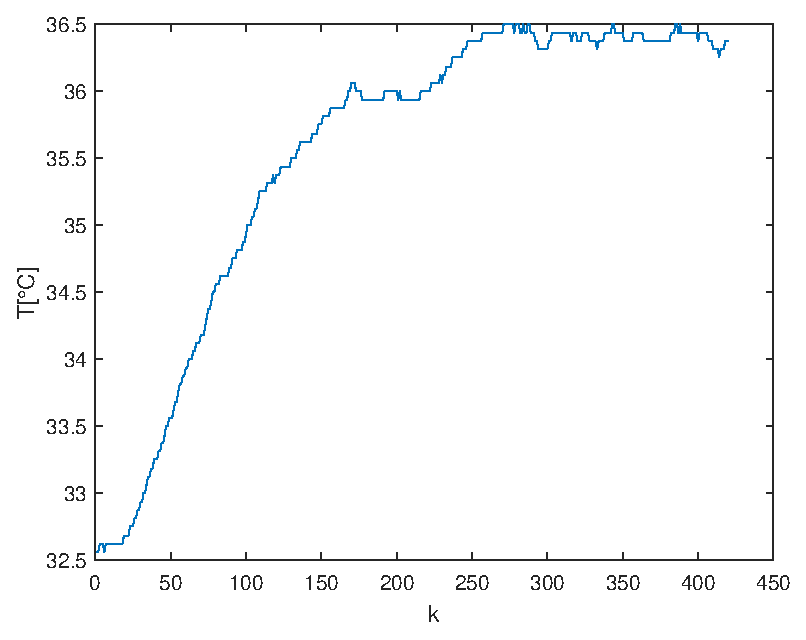
\includegraphics[scale=1]{Rys/Skok20_30.eps}
	\caption{Skok wartości sterowania z 20 do 30}
	\label{skok1}
\end{figure}

\begin{figure}[h!]
	\centering
	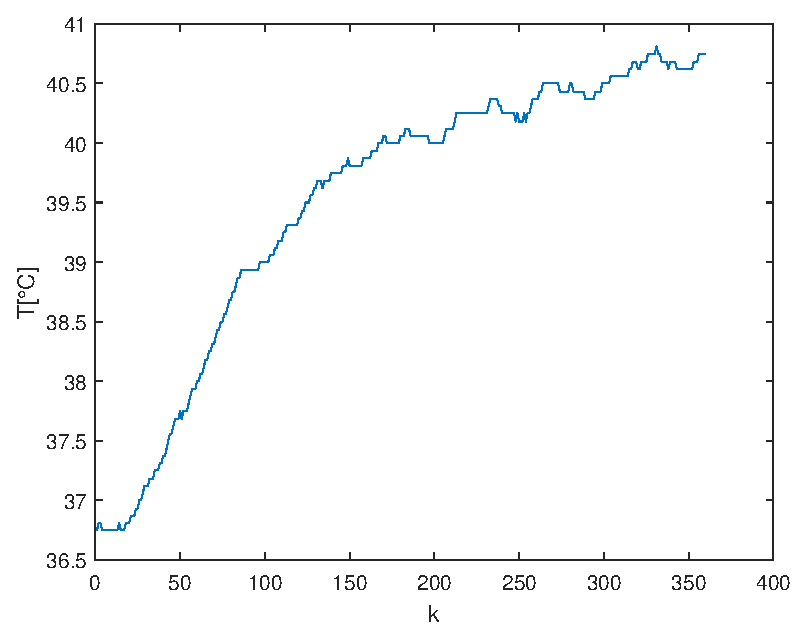
\includegraphics[scale=1]{Rys/Skok30_40.eps}
	\caption{Skok wartości sterowania z 30 do 40}
	\label{skok2}
\end{figure}

\begin{figure}[h!]
	\centering
	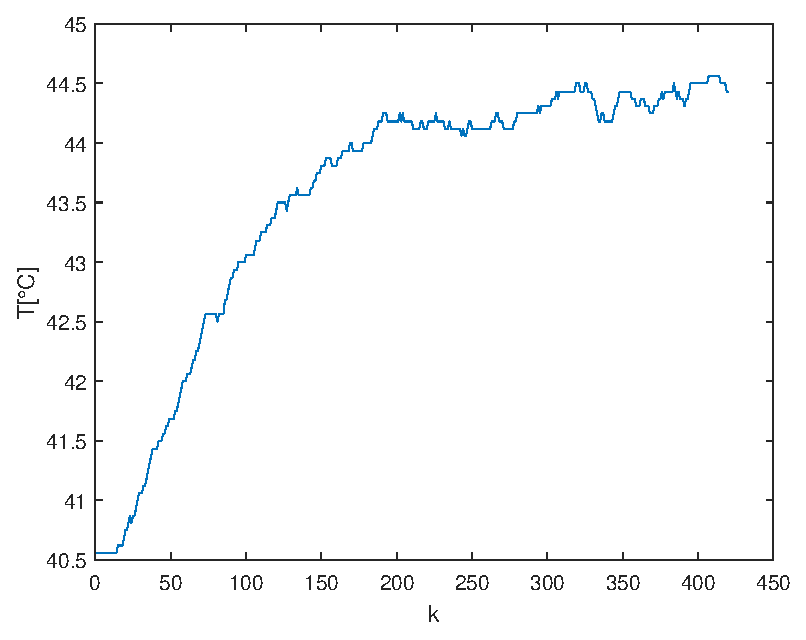
\includegraphics[scale=1]{Rys/Skok40_50.eps}
	\caption{Skok wartości sterowania z 40 do 50}
	\label{skok3}
\end{figure}

\begin{figure}[h!]
	\centering
	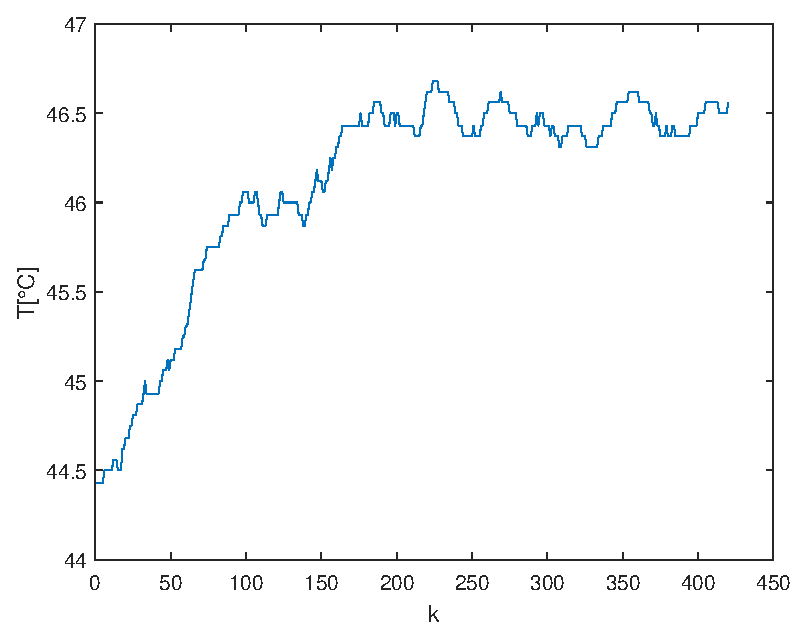
\includegraphics[scale=1]{Rys/Skok50_60.eps}
	\caption{Skok wartości sterowania z 50 do 60}
	\label{skok4}
\end{figure}

\begin{figure}[h!]
	\centering
	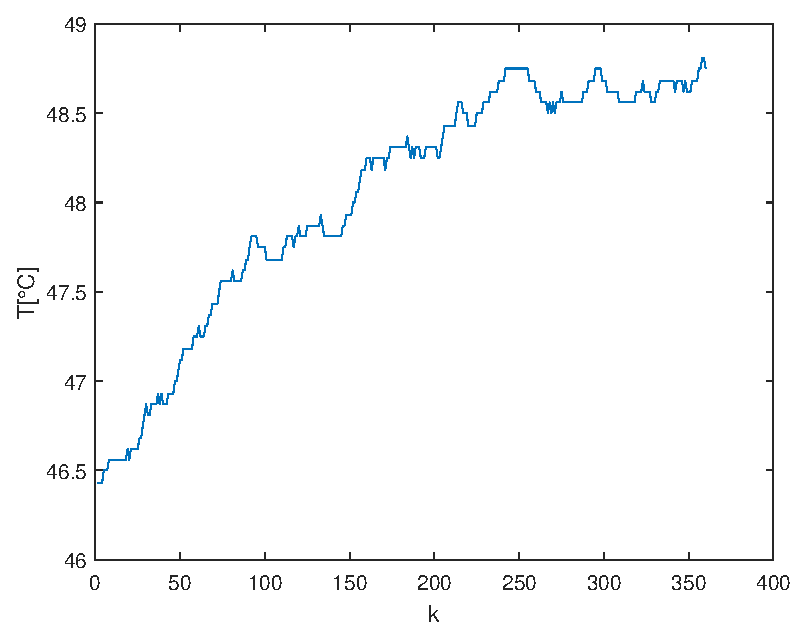
\includegraphics[scale=1]{Rys/Skok60_70.eps}
	\caption{Skok wartości sterowania z 60 do 70}
	\label{skok5}
\end{figure}

\begin{figure}[h!]
	\centering
	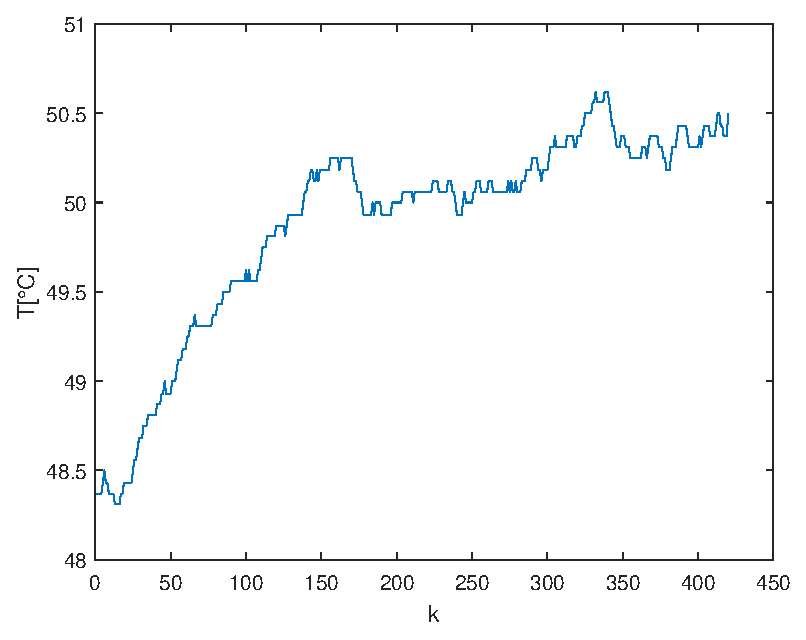
\includegraphics[scale=1]{Rys/Skok70_80.eps}
	\caption{Skok wartości sterowania z 70 do 80}
	\label{skok6}
\end{figure}

\FloatBarrier

Wyniki przedstawiono w tabeli:

\begin{center}
 \begin{tabular}{ | m{1cm}| m{1cm} | }
 \hline
 G1[\%] & T[\degree C]   \\
 \hline
 20 & \num{32,43}   \\ 
 \hline
 30 & \num{36,62 }  \\
 \hline
 40 & \num{40,75}  \\
 \hline
 50 & \num{44,31} \\
 \hline
 60 & \num{46,5}  \\ 
 \hline
 70 & \num{48,68}  \\ 
 \hline
 80 & \num{50,56}  \\
 \hline


\end{tabular}
\end{center}


\section{Charakterystyka statyczna obiektu}

Charakterystykę statyczną obiektu w przedziale sterowań G1 od 20 do 80\% przedstawiono na wykresie \ref{stat}:

\begin{figure}[h!]
	\centering
	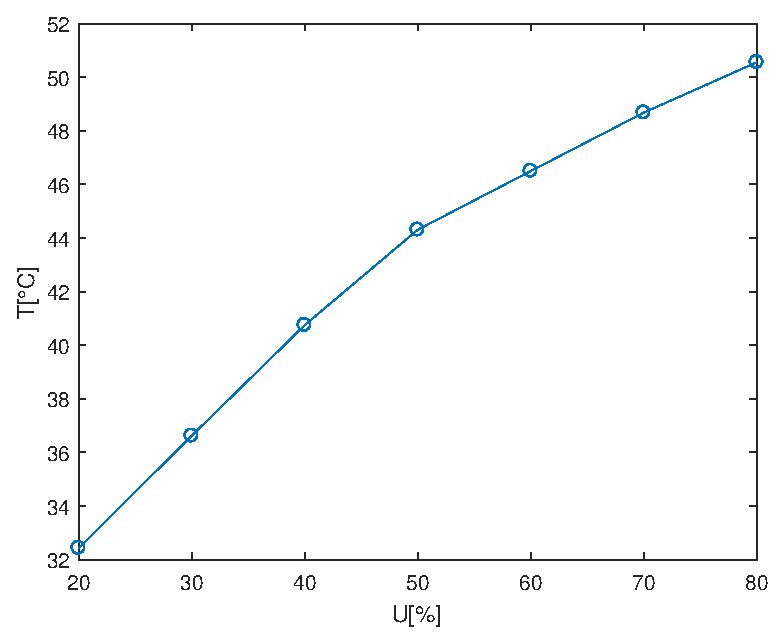
\includegraphics[scale=1]{Rys/Char_stat.eps}
	\caption{Charakterystyka statyczna obiektu}
	\label{stat}
\end{figure}


\section{Wzmocnienie statyczne}

Z wykresu charakterystyki liniowej można stwierdzić, że obiekt nie jest całkowicie liniowy, występuje załamanie charakterystyki w punkcie U=\num{50}\%. Jednak obiekt jest kawałkami liniowy, przejawia właściwości liniowe w przedziale \num{20}-\num{50}\% oraz inne  właściwości liniowe w przedziale \num{50}-\num{80}\% - na tych odcinkach obiekt zachowuje się praktycznie w sposób liniowy. Dlatego też możemy policzyć wzmocnienie statyczne obiektu w tych przedziałach sterowania:

\begin{equation}
K_{\num{20}-\num{50}\%}= \frac{Y(50)-Y(20)}{50-20}=\frac{44,31-32,43}{50-20}=0,396
\label{zad2_wzm_statyczne_wzor1}
\end{equation}


\begin{equation}
K_{\num{50}-\num{80}\%}= \frac{Y(80)-Y(50)}{80-50}=\frac{50,56-44,31}{80-50}\approx 0,208
\label{zad2_wzm_statyczne_wzor2}
\end{equation}


